\chapter{Methods}

\section{Fathi Rabbani / 1164074}
\subsection{Teori}
\begin{enumerate}
\item Random Forest
\subitem
Random forest  adalah suatu algoritma yang digunakan pada klasifikasi data dalam jumlah yang besar. Klasifikasi random forest dilakukan melalui penggabungan pohon (tree) dengan melakukan training pada sampel data yang dimiliki. Penggunaan pohon (tree) yang semakin banyak akan mempengaruhi akurasi yang akan didapatkan menjadi lebih baik. Penentuan klasifikasi dengan random forest diambil berdasarkan hasil voting dari tree yang terbentuk. Pemenang dari tree yang terbentuk ditentukan dengan vote terbanyak. berikut adalah struktur dari Random Forest ada pada Gambar \ref{fig1}

\item Membaca Dataset, Makna setiap file dan Menjelaskan data CUB-200-2011
\begin{enumerate}
\item Membaca Data
\begin{itemize}
\item
dengan membuka data yang sudah didownload yaitu data CUB-200-2011 atau data tentang perbandingan data jenis burung,
\item
lalu data tersebut dibuka dengan menggunakan aplikasi Spyder, dan dijalankan setiap baris Code yang ada.
\item data yang ada pada folder CUB-200-2011 dibuka dengan menggunakan code dari Chapter 2 yang ada pada buku pembelajaran.
\end{itemize}

\item Makna setiap File
\begin{itemize}
\item data yang terdapat pada file CUB-200-2011 ada data folder ATTRIBUTE, IMAGES, PARTS yang memiliki kegunaannya sendiri yang dimana pada penggunaannya data yang dipakai adalah data image\_attribute\_label pada folder attribute, data image\_class\_labels dan data classes.
\item file image\_attribute\_label berguna sebagai data awal yang digunakan untuk membaca data attribute yang terdapat pada masing - masing gambar burung yang ada.
\item sedangkan file image\_class\_label yang ada pada folder CUB-200-2011 berguna sebagai data yang akan membuat kolom baru pada dataset yang fungsinya adalah untuk memasukan hasil dari semua data yang dimiliki oleh imgatt2.
\item dan file classes berguna sebagai dataset yang akan dipanggil oleh fungsi code untuk menampilkan nama dari data burung yang dimiliki.
\end{itemize}

\item Isi Field
\begin{itemize}
\item file image\_attribute\_label
berisi tentang data attribute yang ada pada data gambar file burung yang dimiliki difolder image pada CUB-200-2011
\item file image\_class\_label
berisi tentang data yang dimiliki oleh attribute dari image\_attribute\_label dimana data yang bernilai atau memiliki nilai disusun hingga menghasilkan data yang mudah dipahami.
\item file classes
berisi tentang data yang berguna untuk menampilkan data nama dari setiap data jenis burung yang dimiliki.
\end{itemize}
\end{enumerate}

\item Cross Validation
\subitem
Cross-validation adalah metode statistik yang dapat digunakan untuk mengevaluasi kinerja model atau algoritma dimana data dipisahkan menjadi dua subset yaitu data training dan data testing.

\item Score 44 Random Forest, 27 Decision Tree dan 29 SVM
\begin{enumerate}
\item
merupakan hasil dari pengolahan tentang data jenis burung yang dimiliki setelah melalui proses pembagian data training dan testing yang menghasilkan score 44 persen sebagai pembanding bahwa data yang diolah tersebut bernilai 44 persen tingkat kebenarannya atau keakuratannya.
\item
lalu pada penggunaan decision tree yang menghasilkan nilai 27 persen menjelaskan bahwa data yang diolah dengan menggunakan decision tree sebagai fungsi pembandingannya itu lebih kecil tingkat keakuratan hasilnya yang dimana kita mencari keakuratan data dari setiap jenis burung yang ada.
\item
sedangkan dengan menggunakan SVM menghasilkan nilai sebesar 29 persen yang dimana merupakan nilai nertal menjelaskan bahwa data yang diolah masih belum akurat tingkat kesamaannya dengan data jenis burung yang dimiliki.
\end{enumerate}
dari penjelasan tersebut disimpulkan bahwa penggunaan randowm forest dalam menentukan keakuratan data itu lebih besar scorenya dibandingkan menggunakan decision tree dan SVM.

\item Membaca Confusion Matriks
\begin{verbatim}
import numpy as np
np.set_printoptions(precision=2)
plt.figure(figsize=(60,60), dpi=300)
plot_confusion_matrix(cm, classes=birds, normalize=True)
plt.show()
\end{verbatim}
penggunaan code diatas adala cara untuk membaca dataset jenis burung dengan metode confusion matriks. dimana contoh hasil dari membaca data dengan menggunakan confusion matriks adalah sebagai berikut : Gambar \ref{fig2}

\item Voting pada Random Forest
voting pada random forest berguna untuk mengambil nilai yang akan digunakan sebagai bandingan dari masing - masing tree yang ada untuk menghasilkan nilai final sebagai data yang diinginkan, contohnya adalah seperti berikut ini : Gambar \ref{fig3}
\end{enumerate}

\begin{figure}[ht]
	\centerline{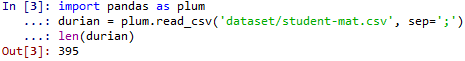
\includegraphics[width=1\textwidth]{figures/fathi/chapter3/1.png}}
	\caption{Random Forest}
	\label{fig1}
\end{figure}

\begin{figure}[ht]
	\centerline{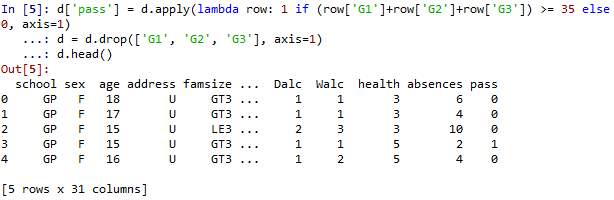
\includegraphics[width=1\textwidth]{figures/fathi/chapter3/2.PNG}}
	\caption{Hasil dari membaca data dengan Confusion Matriks}
	\label{fig2}
\end{figure}

\begin{figure}[ht]
	\centerline{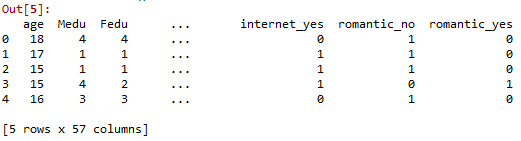
\includegraphics[width=1\textwidth]{figures/fathi/chapter3/3.png}}
	\caption{Voting Random Forest}
	\label{fig3}
\end{figure}